
%% bare_conf.tex
%% V1.3
%% 2007/01/11
%% by Michael Shell
%% See:
%% http://www.michaelshell.org/
%% for current contact information.
%%
%% This is a skeleton file demonstrating the use of IEEEtran.cls
%% (requires IEEEtran.cls version 1.7 or later) with an IEEE conference paper.
%%
%% Support sites:
%% http://www.michaelshell.org/tex/ieeetran/
%% http://www.ctan.org/tex-archive/macros/latex/contrib/IEEEtran/
%% and
%% http://www.ieee.org/

%%*************************************************************************
%% Legal Notice:
%% This code is offered as-is without any warranty either expressed or
%% implied; without even the implied warranty of MERCHANTABILITY or
%% FITNESS FOR A PARTICULAR PURPOSE! 
%% User assumes all risk.
%% In no event shall IEEE or any contributor to this code be liable for
%% any damages or losses, including, but not limited to, incidental,
%% consequential, or any other damages, resulting from the use or misuse
%% of any information contained here.
%%
%% All comments are the opinions of their respective authors and are not
%% necessarily endorsed by the IEEE.
%%
%% This work is distributed under the LaTeX Project Public License (LPPL)
%% ( http://www.latex-project.org/ ) version 1.3, and may be freely used,
%% distributed and modified. A copy of the LPPL, version 1.3, is included
%% in the base LaTeX documentation of all distributions of LaTeX released
%% 2003/12/01 or later.
%% Retain all contribution notices and credits.
%% ** Modified files should be clearly indicated as such, including  **
%% ** renaming them and changing author support contact information. **
%%
%% File list of work: IEEEtran.cls, IEEEtran_HOWTO.pdf, bare_adv.tex,
%%                    bare_conf.tex, bare_jrnl.tex, bare_jrnl_compsoc.tex
%%*************************************************************************

% *** Authors should verify (and, if needed, correct) their LaTeX system  ***
% *** with the testflow diagnostic prior to trusting their LaTeX platform ***
% *** with production work. IEEE's font choices can trigger bugs that do  ***
% *** not appear when using other class files.                            ***
% The testflow support page is at:
% http://www.michaelshell.org/tex/testflow/



% Note that the a4paper option is mainly intended so that authors in
% countries using A4 can easily print to A4 and see how their papers will
% look in print - the typesetting of the document will not typically be
% affected with changes in paper size (but the bottom and side margins will).
% Use the testflow package mentioned above to verify correct handling of
% both paper sizes by the user's LaTeX system.
%
% Also note that the "draftcls" or "draftclsnofoot", not "draft", option
% should be used if it is desired that the figures are to be displayed in
% draft mode.
%
\documentclass[11pt,conference]{IEEEtran}
% Add the compsoc option for Computer Society conferences.
%
% If IEEEtran.cls has not been installed into the LaTeX system files,
% manually specify the path to it like:
% \documentclass[conference]{../sty/IEEEtran}





% Some very useful LaTeX packages include:
% (uncomment the ones you want to load)


% *** MISC UTILITY PACKAGES ***
%
%\usepackage{ifpdf}
% Heiko Oberdiek's ifpdf.sty is very useful if you need conditional
% compilation based on whether the output is pdf or dvi.
% usage:
% \ifpdf
%   % pdf code
% \else
%   % dvi code
% \fi
% The latest version of ifpdf.sty can be obtained from:
% http://www.ctan.org/tex-archive/macros/latex/contrib/oberdiek/
% Also, note that IEEEtran.cls V1.7 and later provides a builtin
% \ifCLASSINFOpdf conditional that works the same way.
% When switching from latex to pdflatex and vice-versa, the compiler may
% have to be run twice to clear warning/error messages.






% *** CITATION PACKAGES ***
%
%\usepackage{cite}
% cite.sty was written by Donald Arseneau
% V1.6 and later of IEEEtran pre-defines the format of the cite.sty package
% \cite{} output to follow that of IEEE. Loading the cite package will
% result in citation numbers being automatically sorted and properly
% "compressed/ranged". e.g., [1], [9], [2], [7], [5], [6] without using
% cite.sty will become [1], [2], [5]--[7], [9] using cite.sty. cite.sty's
% \cite will automatically add leading space, if needed. Use cite.sty's
% noadjust option (cite.sty V3.8 and later) if you want to turn this off.
% cite.sty is already installed on most LaTeX systems. Be sure and use
% version 4.0 (2003-05-27) and later if using hyperref.sty. cite.sty does
% not currently provide for hyperlinked citations.
% The latest version can be obtained at:
% http://www.ctan.org/tex-archive/macros/latex/contrib/cite/
% The documentation is contained in the cite.sty file itself.






% *** GRAPHICS RELATED PACKAGES ***
%
\ifCLASSINFOpdf
  % \usepackage[pdftex]{graphicx}
  % declare the path(s) where your graphic files are
  % \graphicspath{{../pdf/}{../jpeg/}}
  % and their extensions so you won't have to specify these with
  % every instance of \includegraphics
  % \DeclareGraphicsExtensions{.pdf,.jpeg,.png}
\else
  % or other class option (dvipsone, dvipdf, if not using dvips). graphicx
  % will default to the driver specified in the system graphics.cfg if no
  % driver is specified.
  % \usepackage[dvips]{graphicx}
  % declare the path(s) where your graphic files are
  % \graphicspath{{../eps/}}
  % and their extensions so you won't have to specify these with
  % every instance of \includegraphics
  % \DeclareGraphicsExtensions{.eps}
\fi
% graphicx was written by David Carlisle and Sebastian Rahtz. It is
% required if you want graphics, photos, etc. graphicx.sty is already
% installed on most LaTeX systems. The latest version and documentation can
% be obtained at: 
% http://www.ctan.org/tex-archive/macros/latex/required/graphics/
% Another good source of documentation is "Using Imported Graphics in
% LaTeX2e" by Keith Reckdahl which can be found as epslatex.ps or
% epslatex.pdf at: http://www.ctan.org/tex-archive/info/
%
% latex, and pdflatex in dvi mode, support graphics in encapsulated
% postscript (.eps) format. pdflatex in pdf mode supports graphics
% in .pdf, .jpeg, .png and .mps (metapost) formats. Users should ensure
% that all non-photo figures use a vector format (.eps, .pdf, .mps) and
% not a bitmapped formats (.jpeg, .png). IEEE frowns on bitmapped formats
% which can result in "jaggedy"/blurry rendering of lines and letters as
% well as large increases in file sizes.
%
% You can find documentation about the pdfTeX application at:
% http://www.tug.org/applications/pdftex





% *** MATH PACKAGES ***
%
%\usepackage[cmex10]{amsmath}
% A popular package from the American Mathematical Society that provides
% many useful and powerful commands for dealing with mathematics. If using
% it, be sure to load this package with the cmex10 option to ensure that
% only type 1 fonts will utilized at all point sizes. Without this option,
% it is possible that some math symbols, particularly those within
% footnotes, will be rendered in bitmap form which will result in a
% document that can not be IEEE Xplore compliant!
%
% Also, note that the amsmath package sets \interdisplaylinepenalty to 10000
% thus preventing page breaks from occurring within multiline equations. Use:
%\interdisplaylinepenalty=2500
% after loading amsmath to restore such page breaks as IEEEtran.cls normally
% does. amsmath.sty is already installed on most LaTeX systems. The latest
% version and documentation can be obtained at:
% http://www.ctan.org/tex-archive/macros/latex/required/amslatex/math/





% *** SPECIALIZED LIST PACKAGES ***
%
%\usepackage{algorithmic}
% algorithmic.sty was written by Peter Williams and Rogerio Brito.
% This package provides an algorithmic environment fo describing algorithms.
% You can use the algorithmic environment in-text or within a figure
% environment to provide for a floating algorithm. Do NOT use the algorithm
% floating environment provided by algorithm.sty (by the same authors) or
% algorithm2e.sty (by Christophe Fiorio) as IEEE does not use dedicated
% algorithm float types and packages that provide these will not provide
% correct IEEE style captions. The latest version and documentation of
% algorithmic.sty can be obtained at:
% http://www.ctan.org/tex-archive/macros/latex/contrib/algorithms/
% There is also a support site at:
% http://algorithms.berlios.de/index.html
% Also of interest may be the (relatively newer and more customizable)
% algorithmicx.sty package by Szasz Janos:
% http://www.ctan.org/tex-archive/macros/latex/contrib/algorithmicx/




% *** ALIGNMENT PACKAGES ***
%
%\usepackage{array}
% Frank Mittelbach's and David Carlisle's array.sty patches and improves
% the standard LaTeX2e array and tabular environments to provide better
% appearance and additional user controls. As the default LaTeX2e table
% generation code is lacking to the point of almost being broken with
% respect to the quality of the end results, all users are strongly
% advised to use an enhanced (at the very least that provided by array.sty)
% set of table tools. array.sty is already installed on most systems. The
% latest version and documentation can be obtained at:
% http://www.ctan.org/tex-archive/macros/latex/required/tools/


%\usepackage{mdwmath}
%\usepackage{mdwtab}
% Also highly recommended is Mark Wooding's extremely powerful MDW tools,
% especially mdwmath.sty and mdwtab.sty which are used to format equations
% and tables, respectively. The MDWtools set is already installed on most
% LaTeX systems. The lastest version and documentation is available at:
% http://www.ctan.org/tex-archive/macros/latex/contrib/mdwtools/


% IEEEtran contains the IEEEeqnarray family of commands that can be used to
% generate multiline equations as well as matrices, tables, etc., of high
% quality.


%\usepackage{eqparbox}
% Also of notable interest is Scott Pakin's eqparbox package for creating
% (automatically sized) equal width boxes - aka "natural width parboxes".
% Available at:
% http://www.ctan.org/tex-archive/macros/latex/contrib/eqparbox/





% *** SUBFIGURE PACKAGES ***
%\usepackage[tight,footnotesize]{subfigure}
% subfigure.sty was written by Steven Douglas Cochran. This package makes it
% easy to put subfigures in your figures. e.g., "Figure 1a and 1b". For IEEE
% work, it is a good idea to load it with the tight package option to reduce
% the amount of white space around the subfigures. subfigure.sty is already
% installed on most LaTeX systems. The latest version and documentation can
% be obtained at:
% http://www.ctan.org/tex-archive/obsolete/macros/latex/contrib/subfigure/
% subfigure.sty has been superceeded by subfig.sty.



%\usepackage[caption=false]{caption}
%\usepackage[font=footnotesize]{subfig}
% subfig.sty, also written by Steven Douglas Cochran, is the modern
% replacement for subfigure.sty. However, subfig.sty requires and
% automatically loads Axel Sommerfeldt's caption.sty which will override
% IEEEtran.cls handling of captions and this will result in nonIEEE style
% figure/table captions. To prevent this problem, be sure and preload
% caption.sty with its "caption=false" package option. This is will preserve
% IEEEtran.cls handing of captions. Version 1.3 (2005/06/28) and later 
% (recommended due to many improvements over 1.2) of subfig.sty supports
% the caption=false option directly:
%\usepackage[caption=false,font=footnotesize]{subfig}
%
% The latest version and documentation can be obtained at:
% http://www.ctan.org/tex-archive/macros/latex/contrib/subfig/
% The latest version and documentation of caption.sty can be obtained at:
% http://www.ctan.org/tex-archive/macros/latex/contrib/caption/




% *** FLOAT PACKAGES ***
%
%\usepackage{fixltx2e}
% fixltx2e, the successor to the earlier fix2col.sty, was written by
% Frank Mittelbach and David Carlisle. This package corrects a few problems
% in the LaTeX2e kernel, the most notable of which is that in current
% LaTeX2e releases, the ordering of single and double column floats is not
% guaranteed to be preserved. Thus, an unpatched LaTeX2e can allow a
% single column figure to be placed prior to an earlier double column
% figure. The latest version and documentation can be found at:
% http://www.ctan.org/tex-archive/macros/latex/base/



%\usepackage{stfloats}
% stfloats.sty was written by Sigitas Tolusis. This package gives LaTeX2e
% the ability to do double column floats at the bottom of the page as well
% as the top. (e.g., "\begin{figure*}[!b]" is not normally possible in
% LaTeX2e). It also provides a command:
%\fnbelowfloat
% to enable the placement of footnotes below bottom floats (the standard
% LaTeX2e kernel puts them above bottom floats). This is an invasive package
% which rewrites many portions of the LaTeX2e float routines. It may not work
% with other packages that modify the LaTeX2e float routines. The latest
% version and documentation can be obtained at:
% http://www.ctan.org/tex-archive/macros/latex/contrib/sttools/
% Documentation is contained in the stfloats.sty comments as well as in the
% presfull.pdf file. Do not use the stfloats baselinefloat ability as IEEE
% does not allow \baselineskip to stretch. Authors submitting work to the
% IEEE should note that IEEE rarely uses double column equations and
% that authors should try to avoid such use. Do not be tempted to use the
% cuted.sty or midfloat.sty packages (also by Sigitas Tolusis) as IEEE does
% not format its papers in such ways.





% *** PDF, URL AND HYPERLINK PACKAGES ***
%
%\usepackage{url}
% url.sty was written by Donald Arseneau. It provides better support for
% handling and breaking URLs. url.sty is already installed on most LaTeX
% systems. The latest version can be obtained at:
% http://www.ctan.org/tex-archive/macros/latex/contrib/misc/
% Read the url.sty source comments for usage information. Basically,
% \url{my_url_here}.





% *** Do not adjust lengths that control margins, column widths, etc. ***
% *** Do not use packages that alter fonts (such as pslatex).         ***
% There should be no need to do such things with IEEEtran.cls V1.6 and later.
% (Unless specifically asked to do so by the journal or conference you plan
% to submit to, of course. )


% correct bad hyphenation here
\hyphenation{key-strokes}

\usepackage{graphicx}
\usepackage{multirow}

\begin{document}
%
% paper title
% can use linebreaks \\ within to get better formatting as desired
\title{EavesDroid: Keystroke recovery using mobile phone accelerometers}

% author names and affiliations
% use a multiple column layout for up to three different
% affiliations
\author{\IEEEauthorblockN{Jennifer Guo}
\IEEEauthorblockA{Princeton University}
%Georgia Institute of Technology\\
%Atlanta, Georgia 30332--0250\\
%Email: http://www.michaelshell.org/contact.html}
\and
\IEEEauthorblockN{Yi-Hsien Lin}
\IEEEauthorblockA{Princeton University}
\and
\IEEEauthorblockN{Akshay Mittal}
\IEEEauthorblockA{Princeton University}
\and
\IEEEauthorblockN{Wathsala Vithanage}
\IEEEauthorblockA{Princeton University}
}

% conference papers do not typically use \thanks and this command
% is locked out in conference mode. If really needed, such as for
% the acknowledgment of grants, issue a \IEEEoverridecommandlockouts
% after \documentclass

% for over three affiliations, or if they all won't fit within the width
% of the page, use this alternative format:
% 
%\author{\IEEEauthorblockN{Michael Shell\IEEEauthorrefmark{1},
%Homer Simpson\IEEEauthorrefmark{2},
%James Kirk\IEEEauthorrefmark{3}, 
%Montgomery Scott\IEEEauthorrefmark{3} and
%Eldon Tyrell\IEEEauthorrefmark{4}}
%\IEEEauthorblockA{\IEEEauthorrefmark{1}School of Electrical and Computer Engineering\\
%Georgia Institute of Technology,
%Atlanta, Georgia 30332--0250\\ Email: see http://www.michaelshell.org/contact.html}
%\IEEEauthorblockA{\IEEEauthorrefmark{2}Twentieth Century Fox, Springfield, USA\\
%Email: homer@thesimpsons.com}
%\IEEEauthorblockA{\IEEEauthorrefmark{3}Starfleet Academy, San Francisco, California 96678-2391\\
%Telephone: (800) 555--1212, Fax: (888) 555--1212}
%\IEEEauthorblockA{\IEEEauthorrefmark{4}Tyrell Inc., 123 Replicant Street, Los Angeles, California 90210--4321}}




% use for special paper notices
%\IEEEspecialpapernotice{(Invited Paper)}




% make the title area
\maketitle


\begin{abstract}
%\boldmath
[to - fill]
\end{abstract}
% IEEEtran.cls defaults to using nonbold math in the Abstract.
% This preserves the distinction between vectors and scalars. However,
% if the conference you are submitting to favors bold math in the abstract,
% then you can use LaTeX's standard command \boldmath at the very start
% of the abstract to achieve this. Many IEEE journals/conferences frown on
% math in the abstract anyway.

% no keywords




% For peer review papers, you can put extra information on the cover
% page as needed:
% \ifCLASSOPTIONpeerreview
% \begin{center} \bfseries EDICS Category: 3-BBND \end{center}
% \fi
%
% For peerreview papers, this IEEEtran command inserts a page break and
% creates the second title. It will be ignored for other modes.
\IEEEpeerreviewmaketitle



\section{Introduction}
% no \IEEEPARstart
\label{sec:introduction}
\noindent Mobile phones are becoming increasingly powerful
devices. In addition to being able to run simple applications such as email clients and web browsers; by equipping a wide variety of sophisticated sensors, these smartphones can actively interface with the world around them.

Unfortunately, the array of sensors in these devices can also be
used in malicious ways. For example, malware could
potentially gain access to a mobile phone's camera to take photos or
video without the notice of the owner \cite{cheng2007mobile}. Other possible attempts are activating the device's microphone to record converstaions or turn on the GPS to track the target's position
\cite{dagon2004mobile, cai2009defending, enck2010taintdroid, egele2011pios}.
In light of the possible privacy threats mentioned above, operating systems that are implemented in modern mobile phones usually provide mechanisms so that applications must acquire the user's explicit permission before it can access the device's sensors.

For instance, an Android application would have a manifest file that includes a list of all permissions an application can request during installation time. Under this design, the application is either granted a particular permission when installed, and can use that feature as desired, or the permission is not granted and any attempt to use the feature fails without prompting the user. However, not all sensors' accesses are tightly regulated by this mechanism, which leads to several potential sensors abuse.


One such example is the accelerometer. Access to accelerometers are usually un-restricted on most of the current mobile phone operating systems. In this paper, we developed \textbf{EavesDroid}, which is a malicious application with access to the accelerometer's data. We demonstrate that \textbf{EavesDroid} is able to record and reconstruct the keypresses made on a nearby keyboard with decent accuracy, based solely on the observed vibrations. We develop profiles for keypress by extracing features from the keypress signals and classifies them using boosted Random Forests. This allows us to establish an abstract representation of the relationship between a keystroke signal and its corresponding key. We then recover the typed content
by translating from our intermediary form to English words using a number
of different dictionaries. As mentioned in \cite{spiphone}, reconstructing keystrokes from vibration signals is very different and much more difficult from previous efforts in this space since they are mostly based on acoustic or electromagnetic eavesdropping and enjoys a higher sampling rate. 

By developing \textbf{EavesDroid} we have made the following contributions to the smarphone security domain:
\begin{enumerate}
\item {\bf Develop an infrastructure for characterizing keypress vibrations}: We
capture, analyze and develop profiles of keypress events on a nearby
keyboard based on the vibrations created when they are pressed. Features such as mean, skewness and FFT are first extracted from our input signals. We then use a set boosted Random Forests to create an intermediary
representation, which is combined with candidate dictionaries
to successfully recover words at rates as high as \_\_ %.
\item {\bf Dataset made publicly available}: To the best of our knowledge,
there does not exists a dataset with
the keystrokes for the vibrations recorded using an accelerometer. In this
paper, we demonstrate we construct the dataset of keystroke vibrations,
recorded using the accelerometer, present in a smartphone and make
the dataset publicly available to enhance further research on this topic. Given
the widespread about security breaches and email leaks, we perceive this to be
of great importance in motivating the mobile operating system manufacturers
to restrict the usage of accelerometers to permitted applications only.\\
\end{enumerate}
\noindent Note that our approach is greatly influenced by the work of
Marquardt \emph{et. al}~\cite{spiphone} and we present key differences with our
approach.

\section{Related Work}
\noindent Researchers have studied malicious code on mobile devices that
learn information about the device owner using other embedded sensors.
In the most closely related work to our paper, Marquardt \emph{et. al}
\cite{spiphone} propose \emph{(sp)iPhone} which uses motion sensors in the
iPhone 4
to infer keystrokes of nearby laptop users. \emph{(sp)iPhone} uses 3 labels for
each pair of keystrokes in order to determine the correct identification for
the letters of the word. The location of the key is modelled using a neural
network trained on 150 keystrokes for each letter of the English alphabet.
A profile is then constructed for each pair using the neural network and
determines and models the distance between the two events. The predictions
of the neural network are matched against a dictionary to determine the top
matches. The accuracy achieved is roughly 80\% but this decreases to 40\%
as the size of the dictionary increases.

In a very similar, but orthogonal, use case, Owusu \emph{et. al}
\cite{owusu2012accessory}
present the threat of applications which extract the keystrokes of the
user's typing on the smartphone screen itself. Again, due to no restrictions
on the usage of the accelerometer, they are able to extract 6-character
passwords in as few as 4.5 trials(median). TouchLogger~\cite{cai2011touchlogger}
uses orientation of the smartphone device to infer the keystrokes.

\section{Threat Model}
\noindent Our attack is based upon two observations:

Different from most of the sensors on a smartphone such as microphone, camera and GPS, the access of the accelerometer is not protected by the permission mechanism mentioned earlier. That is to say, any application is able to access the accelerometer feed if they wish to. However, due to the frequent usage needs of the accelerometer to determine window orientation and update screen orientation, we envision that this problem will not be fixed in the near future. Therefore, the number of smartphone that are vulnerable to this threat will only increase in the near future.

Our second observation is that smartphones are often placed very closely to a laptop or the keyboard of a computer. This is mainly because smartphone users tends to put their phone within their reaching area while working so they can monitor the phone should any text or notifications pops up. Therefore, this behaviour enables the accelerometer within the smartphone to record clear keystroke signals before they diminish and get corrupted. This clearly exacerbates the threat that accelerometer data is not protected since malicious applications such as \textbf{EavesDroid} would have access to more distinguishable signals


\section{Framework Description}

\subsection{Dataset Capturing}
\label{sec:dataset-capturing}
\noindent Our experimental setup is shown in Figure~\ref{fig:setup}. We placed a Dell USB keyboard and a LG Nexus 5 smartphone on a wooden table. No other items were placed on or were touching the table. All keys were pressed with the index finger of the right hand. The hands do not touch the keyboard or table, and the fingers do not pause on the keyboard but only touch it during the brief duration of the key press.

We recorded 1000 data points in 40 sessions with 25 letters in each sessions. For each session we generate a sequence of 25 random letters and display the letters in 3 second intervals to ensure an even recording of the letters and to ensure that there is no bias toward a specific letter. For the data capturing we developed an Android app that reads from the hardware accelerometer and syncs with our laptops, where we further process the data. The raw accelerometer data as returned by Android contains the $x$, $y$ and $z$-direction components of the acceleration of the vibration received. We calculate the G-force magnitude as $\sqrt{x^2+y^2+z^2}-g$ where $g = 9.81 m/s^2$ is the acceleration due to gravity. The accelerometer records at the granularity of microseconds.

\noindent Figure~\ref{fig:signal-a},~\ref{fig:signal-b} and~\ref{fig:signal-p} show the G-Force values varying with time for the
letters `a', `b' and `p' respectively. It is clear from the plots that there is significant different between the features
of the signal for the different letters and we aim to exploit this difference to recover the typed letters by a user.
Note that the original recordings (not shown in the interest of space) contain a large spike at the beginning and end
due to the pressing of ``Start" and ``Stop" buttons on the recording app.
Therefore, we wrote a module, Clipper, to cut off these noise signals and further segment the data into 25 individual data points.
We will elaborate on this in Section~\ref{sec:learning}.

\subsection{Feature Extraction}
\label{sec:feature-extractor}
Before actually classifying the signals, we first need to extract the features that can best represent the attributes of the signal.  We used a combination of time-domain and frequency-domain features that was mentioned in \cite{spiphone} to construct our feature vector. The time-domain features we calculated includes mean, root mean square (rms), skewness, variance, and kurtosis. As for the frequency-domain feature, we calculated 30 FFT feature in order to represent the frequency attribute of a signal. At the end of this step, we have acqured 40 feature vectors, for each corresponding english letters.

\subsection{L/R, U/D and Triads}
\label{sec:labeler}
For each english letters, we assign it with two different labels which are \emph{Left/Right} (L/R) and \emph{Up/Down} (U/D) respectively. The \emph{Left/Right} label indicates whether the received signal belongs to a key that is on the left or right hemisphere of the keyboard. Keys that are at the left of key (including) \emph{T, G, H} are labeled as \emph{Left} and \emph{Right} otherwise. As for \emph{Up/Down} labels, it indicates whether a signal is associated with a key that belongs to the upper region of the keyboard or the lower region. Keys that belongs to the row of Q-P are labeled as \emph{Up} and \emph{Down} otherwise.\\

In addition to L/R, U/D labels, we also tried to group different keys together in order to lower the classification space. We made the assumption that keys that are close to each other generates similar vibration signals. Therefore, keys were grouped into triads (with one in pairs) based on their location and labeled with their corresponding group number. Following is the group that each keys belongs to:
\{qwa\}-1, \{szx\}-2, \{erd\}-3, \{fcv\}-4, \{tyg\}-5, \{hbn\}-6, \{uij\}-7, \{pol\}-8, \{km\}-9.

\section{Analysis \& Implementation}
\label{sec:implementation}
\noindent In~\cite{spiphone}, Marquardt \emph{et. al} use a neural network to build the signal profiles of the letters typed by the user. We present the implementation details of the algorithms used in order to best generate a prediction model on the training. The given dataset is broken into training (66\%) and testing (33\%) sets. We then generate the prediction model by 10-fold cross-validation on the training set. We use AdaBoost with Random Forests as the weak learner, AdaBoost with Decision Stumps as the weak learner, and Neural networks to determine the accuracies of the respective models on the testing set (shown in Table~\ref{tab:algos-compare}). The results corresponding to Random Forests are using 10 decision trees. The accuracy of using Decision Stump is better than that of Random Forests because of overfitting happening taking place in the Random Forests. When the number of the number of trees in the Random Forests was increased, the training error decreases and the test error increases. Since Random Forests represent a multitude of decision trees, the higher number of trees increases the testing error. On the other hand, Decision Stumps are one node trees and are less prone to overfitting on the training data and provide the similar accuracies as Random Forests with less complex hypotheses/model. Neural Networks achieves almost similar accuracies as the AdaBoost implementations, but we do not use this as our choice of algorithm for the experimentations (Section~\ref{sec:experimentation}). This is because firstly we do not have the MFCCs features extracted from the keystroke signal and these which provides better representation of cepstral information about the signal and capture by the neural network. Secondly, Marquardt \emph{et. al} have presented a solution to the threat model using neural networks and in order to benefit the research community, we attempt to provide an orthogonal analysis with less features and using a different machine learning approach.

The cepstral features corresponding to the FFTs have significant impact on the predictions of the model. Table~\ref{tab:ffts-non-ffts} shows the test accuracies using AdaBoost with Decision Stumps. FFTs alone provide 10\% higher correct predictions compared to the rest of the features in the case of LR dataset. The combined prediction accuracy when using all the features is better than when using just the FFTs and this demonstrates that the frequency of the vibration signal received from the different keystrokes has significant impact in making correct alphabet predictions.

In addition to LR and UD datasets, we compute the predictions of the algorithms on the Triads dataset. Table~\ref{tab:algos-compare} shows that the models generated make poor predictions about the triad to which a keystroke belongs. This is, firstly, due to the assumption that the alphabets grouped into the same triad do not necessarily have similar keystroke vibrations. Careful triads construction is expected to give better predictions but this is analysis is beyond the scope of this project study and we leave it as future work in the interest of limited time for this project. Therefore, for the purpose of experimentation, we use LR and UD label predictions only for determining the keystrokes of the user. Section~\ref{sec:experimentation} will demonstrate that good triad predictions, in addition to LR and UD predictions, will increase the accuracy with which the words typed by the user are identified. 

\section{Framework Work Flow}
\label{sec:framework}
\noindent In this section, we aim to elaborate the flow of data and features leading to the
predictions made by the model.
\subsection{Learning Phase}
\label{sec:learning}
\noindent In the learning phase (Figure-REF), we use the 1000 data points collected (Section~\ref{sec:dataset-capturing})
for training the model. Each session of the collected data results in one raw accelerometer readings' file.
Since the readings have noise peaks at the start and end of the signal, it is passed through the Clipper
which strips out the ends. The clipped file is then processed by the SignalBreaker to
get the raw accelerometer data for the letters that constitute the session. The segregated letter files are used
to generate two labeled datasets - L/R labels and U/D labels - for the letters. This allows for generating two
trained models in the learning. The labeled letters are passed through the Feature Extractor module
(Section~\ref{sec:feature-extractor}) to the get the labeled
feature vectors. This is followed by the supervised learning of the AdaBoost classifier which Decision Stumps
as the weak learners on the labeled feature vectors and giving the two models for L/R classifier and
the UD classifier.

\subsection{Attack Phase}
\label{sec:attacking}
\noindent In the attack phase (Figure-REF), EavesDroid receives the raw accelerometer data for a word
typed in by the user on a nearby keyboard. The clipping of the signal and signal breaking
works in the same manner as in the learning phase except there is no labeling in the attack
phase. The unlabeled features obtained from the Feature Extractor module are passed
to the classifiers (obtained from the learning phase) and the L/R and UD label predictions
are obtained. The attack module also takes in LR and UD labeled dictionary words from the
72 Harvard sentences. The feature matching module, in the attack module, gives the top
$k$ closest matching words corresponding to the raw accelerometer data received by EavesDroid.

\section{Experimentation}
\label{sec:experimentation}
\noindent We extensively use the R Project~\cite{r-project} tool for collecting the
cepstral features from the data and building the prediction models. R Project
provides access to the RWeka~\cite{rweka} library which has implementations
of most machine learning algorithms. The AdaBoost and Neural Networks implementations
are leveraged from the RWeka package for the purpose of the experiments.

We demonstrate the accuracies of our prediction model on the Harvard
sentences~\cite{harvard-sentences}. We chose this list of sentences because
it is phonetically-balanced, \emph{i.e.} it uses specific English phonemes
with a uniform distribution. For testing the accuracy of text recovery when
a user types on the near-by keyboard, we wrote a module, SignalBreaker, to break the vibration
signal received corresponding to each word into corresponding set of letters for
the particular word. There is a distinct peak corresponding to each key press and
the duration of a keypress is approximately 100ms~\cite{spiphone}. SignalBreaker
uses this information to create segments. It achieves an accuracy of 100\% in
determining the peaks and constructing the letter signals from the corresponding word
signal. To test the accuracies of the L/R and U/D classifiers, the letter signals
for an unknown word signal are fed to the classifiers. The L/R and U/D predictions
from the classifiers are matched against the dictionary and the closest matching
words are predicted as possibilities. The automation of this process, from typing
of a word (from a sentence) and matching the occurrence of the typed word in the
predicted words, is a non-trivial task and requires an extensive time beyond the scope
of this project study.

We provide a hack around this by exploiting the results that
the SignalBreaker works with 100\% accuracy and that $1/3^{rd}$ of the recorded
alphabet signals (Section~\ref{sec:dataset-capturing}) are unseen by the classifiers.
For any sequence of words, we wrote a module, SignalGen, which generates the possible
signal for that word from the remaining $1/3^{rd}$ of the recorded alphabet signals.
This is done by randomly picking a signal corresponding to each letter of the word
and concatenating them together to form the word signal. For example, for the word
``juice", the signals corresponding to `j', `u', `i', `c', `e' are chosen randomly
from the corresponding unseen signals for those letters. Thus we can now automate
the process of testing the classifiers by feeding large articles to SignalGen
and generating predictions for the corresponding words.

Using the SignalGen module, we 
 


[Box sentence: exact matches and possible choices for non-exact matches]

[Negative analysis, word watch, many potential matches  when dictionary size increases]


\section{Conclusions}

\subsection{Future Work}

Mobile browsers having allowing access to accelerometer data,

http://blogs.adobe.com/cantrell/archives/2012/03/accessing-the-accelerometer-and-gyroscope-in-javascript.html

http://isthisanearthquake.com/

http://isthisanearthquake.com/seismograph.html


%%%%%%%%%%%%% Figures and Tables %%%%%%%%%%%%%%%%%%%%
\begin{figure}
\centering
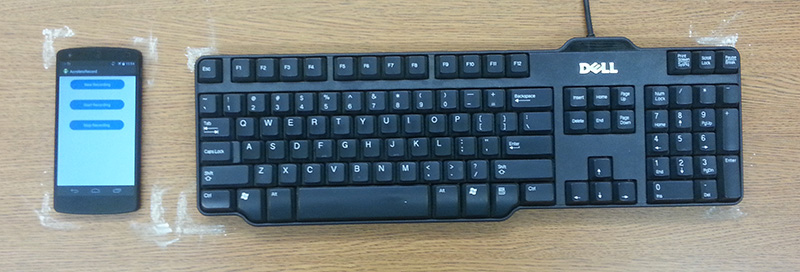
\includegraphics[width=0.5\textwidth]{img/setup}
\caption{Threat model of a smartphone placed next to a keyboard. Used in our experimental setup to capture the dataset.
}
\label{fig:setup}
\end{figure}

\begin{figure}
\centering
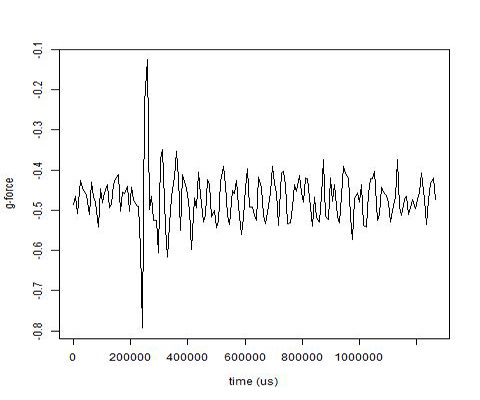
\includegraphics[width=0.5\textwidth]{img/a_162}
\caption{Sample Recording for letter 'a'}
\label{fig:signal-a}
\end{figure}

\begin{figure}
\centering
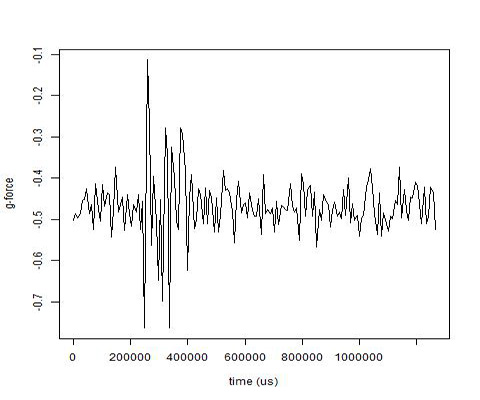
\includegraphics[width=0.5\textwidth]{img/b_147}
\caption{Sample Recording for letter 'b'}
\label{fig:signal-b}
\end{figure}

\begin{figure}
\centering
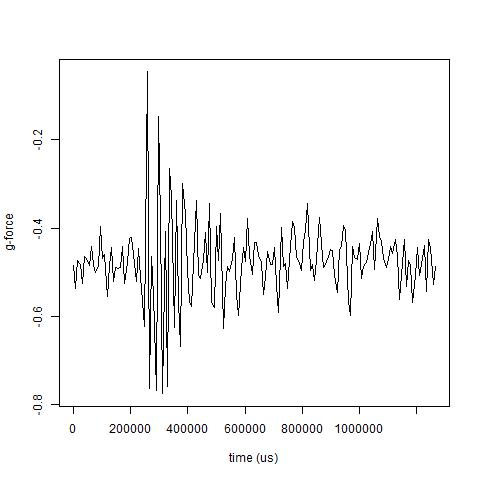
\includegraphics[width=0.5\textwidth]{img/p_566}
\caption{Sample Recording for letter 'p'}
\label{fig:signal-p}
\end{figure}

\begin{table}[h]
\centering
{%\small
\resizebox{8cm}{!}{
\begin{tabular}{|c|c|c|}
\hline
\textbf{Dataset} & \textbf{Algorithm} & \textbf{Test Accuracy(\%)}\\
\hline
\multirow{3}{*}{LR} & AdaBoost (RandomForests) & 68.67\\
\cline{2-3}
& AdaBoost (DecisionStumps) & 69.82\\
\cline{2-3}
& Neural Networks & 68.10\\
\hline
\multirow{3}{*}{UD} & AdaBoost (RandomForests) & 56.60\\
\cline{2-3}
& AdaBoost (DecisionStumps) & 58.68\\
\cline{2-3}
& Neural Networks & 58.62\\
\hline
\multirow{3}{*}{Triads} & AdaBoost (RandomForests) & 16.37\\
\cline{2-3}
& AdaBoost (DecisionStumps) & 13.21\\
\cline{2-3}
& Neural Networks & 14.65\\
\hline
\end{tabular}
}
}
\caption{Test accuracies on $1/3^{rd}$ of dataset}
\label{tab:algos-compare}
\end{table}

\begin{table}[h]
\centering
{%\small
\resizebox{8cm}{!}{
\begin{tabular}{|c|c|c|}
\hline
\textbf{Dataset} & \textbf{Features Picked} & \textbf{Test Accuracy(\%)}\\
\hline
\multirow{2}{*}{LR} & FFTs & 69.54\\
\cline{2-3}
& non-FFTs & 59.48\\
\hline
\multirow{2}{*}{UD} & FFTs & 56.89\\
\cline{2-3}
& non-FFTs & 59.48\\
\hline
\multirow{2}{*}{Triads} & FFTs & 19.54\\
\cline{2-3}
& non-FFTs & 15.22\\
\hline
\end{tabular}
}
}
\caption{Test accuracies with and without FFT features using AdaBoost with RandomForests.}
\label{tab:ffts-non-ffts}
\end{table}

%ACKNOWLEDGMENTS are optional
\section*{Acknowledgments}

% An example of a floating figure using the graphicx package.
% Note that \label must occur AFTER (or within) \caption.
% For figures, \caption should occur after the \includegraphics.
% Note that IEEEtran v1.7 and later has special internal code that
% is designed to preserve the operation of \label within \caption
% even when the captionsoff option is in effect. However, because
% of issues like this, it may be the safest practice to put all your
% \label just after \caption rather than within \caption{}.
%
% Reminder: the "draftcls" or "draftclsnofoot", not "draft", class
% option should be used if it is desired that the figures are to be
% displayed while in draft mode.
%
%\begin{figure}[!t]
%\centering
%\includegraphics[width=2.5in]{myfigure}
% where an .eps filename suffix will be assumed under latex, 
% and a .pdf suffix will be assumed for pdflatex; or what has been declared
% via \DeclareGraphicsExtensions.
%\caption{Simulation Results}
%\label{fig_sim}
%\end{figure}

% Note that IEEE typically puts floats only at the top, even when this
% results in a large percentage of a column being occupied by floats.


% An example of a double column floating figure using two subfigures.
% (The subfig.sty package must be loaded for this to work.)
% The subfigure \label commands are set within each subfloat command, the
% \label for the overall figure must come after \caption.
% \hfil must be used as a separator to get equal spacing.
% The subfigure.sty package works much the same way, except \subfigure is
% used instead of \subfloat.
%
%\begin{figure*}[!t]
%\centerline{\subfloat[Case I]\includegraphics[width=2.5in]{subfigcase1}%
%\label{fig_first_case}}
%\hfil
%\subfloat[Case II]{\includegraphics[width=2.5in]{subfigcase2}%
%\label{fig_second_case}}}
%\caption{Simulation results}
%\label{fig_sim}
%\end{figure*}
%
% Note that often IEEE papers with subfigures do not employ subfigure
% captions (using the optional argument to \subfloat), but instead will
% reference/describe all of them (a), (b), etc., within the main caption.


% An example of a floating table. Note that, for IEEE style tables, the 
% \caption command should come BEFORE the table. Table text will default to
% \footnotesize as IEEE normally uses this smaller font for tables.
% The \label must come after \caption as always.
%
%\begin{table}[!t]
%% increase table row spacing, adjust to taste
%\renewcommand{\arraystretch}{1.3}
% if using array.sty, it might be a good idea to tweak the value of
% \extrarowheight as needed to properly center the text within the cells
%\caption{An Example of a Table}
%\label{table_example}
%\centering
%% Some packages, such as MDW tools, offer better commands for making tables
%% than the plain LaTeX2e tabular which is used here.
%\begin{tabular}{|c||c|}
%\hline
%One & Two\\
%\hline
%Three & Four\\
%\hline
%\end{tabular}
%\end{table}


% Note that IEEE does not put floats in the very first column - or typically
% anywhere on the first page for that matter. Also, in-text middle ("here")
% positioning is not used. Most IEEE journals/conferences use top floats
% exclusively. Note that, LaTeX2e, unlike IEEE journals/conferences, places
% footnotes above bottom floats. This can be corrected via the \fnbelowfloat
% command of the stfloats package.


% conference papers do not normally have an appendix


% trigger a \newpage just before the given reference
% number - used to balance the columns on the last page
% adjust value as needed - may need to be readjusted if
% the document is modified later
%\IEEEtriggeratref{8}
% The "triggered" command can be changed if desired:
%\IEEEtriggercmd{\enlargethispage{-5in}}

% references section

% can use a bibliography generated by BibTeX as a .bbl file
% BibTeX documentation can be easily obtained at:
% http://www.ctan.org/tex-archive/biblio/bibtex/contrib/doc/
% The IEEEtran BibTeX style support page is at:
% http://www.michaelshell.org/tex/ieeetran/bibtex/
%\bibliographystyle{IEEEtran}
% argument is your BibTeX string definitions and bibliography database(s)
%\bibliography{IEEEabrv,../bib/paper}
%
% <OR> manually copy in the resultant .bbl file
% set second argument of \begin to the number of references
% (used to reserve space for the reference number labels box)
\bibliographystyle{unsrt}
\bibliography{sigproc}

%\begin{thebibliography}{1}
%
%\bibitem{IEEEhowto:kopka}
%H.~Kopka and P.~W. Daly, \emph{A Guide to \LaTeX}, 3rd~ed.\hskip 1em plus
%  0.5em minus 0.4em\relax Harlow, England: Addison-Wesley, 1999.
%
%\end{thebibliography}
\appendix
%Appendix A

\section{Appendix Section}

\subsection{Appendix Subsection}

%\balancecolumns




% that's all folks
\end{document}


